\documentclass{book}

%% Math font options
% \usepackage[math]{iwona}
% \usepackage[math]{kurier}
% \usepackage{cmbright}
% \usepackage{lmodern}

%% Font-y stuff
\usepackage{siunitx}
\usepackage{dingbat}
\usepackage[T1]{fontenc}
\usepackage[utf8]{inputenc}
\usepackage{amsfonts}
\usepackage{textcomp}
\usepackage{newtxmath} % Better math lettering (v vs u)


\usepackage{amsmath}

\usepackage{needspace}
%\usepackage{pgfplots}
\usepackage{mdframed}
\usepackage{placeins} % Give float barriers

\usepackage{makeidx}

\usepackage{array} % custom column cells
\newcolumntype{M}[1]{>{\centering\arraybackslash}m{#1}}
\setlength{\tabcolsep}{1em}
\renewcommand{\arraystretch}{1.6}


% Booksize
% \usepackage[top=1in,bottom=0.5in,left=0.5in,right=0.5in,paperwidth=8.5in,paperheight=11in]{geometry}
\usepackage[top=1in,bottom=0.5in,left=0.5in,right=0.5in,paperwidth=7.5in,paperheight=9.25in]{geometry}

% Better Hyphenation
\usepackage[none]{hyphenat}
\usepackage[english]{babel} % Prevents underscore from causing problems with tex4ht 
% Graphics
\usepackage{graphicx}
\usepackage{xcolor}
\usepackage{maxiplot} % Maxima interface

\makeatletter
\@ifpackageloaded{tex4ht}{
\newcommand{\forebook}[1]{#1}
\newcommand{\forprintbook}[1]{}
}{
\newcommand{\forebook}[1]{}
\newcommand{\forprintbook}[1]{#1}
}
\makeatother


\setcounter{tocdepth}{1} % TOC to section level
\setlength{\parindent}{0in} % No paragraph indents
\setlength{\parskip}{10pt} % Between-paragraph skips


\forprintbook{
\def\bookpart#1{%
  \par\newpage\cleardoublepage % Page break
  \thispagestyle{empty}
  \chaptermark{~}
  \sectionmark{~}
  \markboth{~}{~}
  \vspace*{1in} % Vertical shift
  \refstepcounter{part}% Next part
  {\centering\textbf{\Huge Part \thepart}\par}% 
  \addcontentsline{toc}{part}{{\thepart}~~~~~#1}
  \vspace{1cm}% Vertical shift
  {\centering \textbf{\Huge #1}\par}%
  \vspace{2cm}% Vertical shift
  % Some text
}
}

\forebook{
\def\bookpart#1{%
%\section*{~}
%\refstepcounter{part}% Next part
%{\centering\textbf{\Huge Part \thepart}\par}% 
% \part{#1}
% \addcontentsline{toc}{part}{{\thepart}~~~~~#1}
}
}

\forprintbook{
\newenvironment{partintro}{\begin{mdframed}[backgroundcolor=gray!10,skipabove=\baselineskip,skipbelow=\baselineskip]%
~\\ 
}{%
~\\
\end{mdframed}
}
}

\forebook{
\newenvironment{partintro}{}{}
}


% \pgfplotsset{compat=1.10}

\newcommand{\booktitle}[1]{\emph{#1}}

\newcommand{\deriv}[1]{\mathrm{d}#1}
\newcommand{\pd}[2]{\partial{#1}_{#2}}
\newcommand{\myint}{\int\!}
\renewcommand{\dh}{\deriv{h}}
\newcommand{\dx}{\deriv{x}}
\newcommand{\dy}{\deriv{y}}
\newcommand{\ds}{\deriv{s}}
\newcommand{\dr}{\deriv{r}}
\newcommand{\dt}{\deriv{t}}
\newcommand{\du}{\deriv{u}}
\newcommand{\dv}{\deriv{v}}
\newcommand{\dw}{\deriv{w}}
\newcommand{\diff}{\mathrm{d}}
\newcommand{\dz}{\deriv{z}}
\newcommand{\dq}{\deriv{q}}
\newcommand{\dydx}{\frac{\dy}{\dx}}
\newcommand{\arccot}{\mathrm{arccot}}
\newcommand{\arcsec}{\mathrm{arcsec}}
\newcommand{\arccsc}{\mathrm{arccsc}}
\newcommand{\glossterm}[1]{\textbf{#1}}
\newcommand{\fixme}[1]{FIXME---\textbf{#1}}
\newcommand{\degrees}{^{\circ}}


\newcommand{\icode}[1]{\texttt{#1}}

\newcommand\simplegraphicsfigure[3]{
\begin{figure}
\caption{#1}
\label{fig#2}
\centering
\includegraphics[scale=#3]{#2.png}
\end{figure}
}

\newcommand\simplegraph[1]{
	\begin{tikzpicture}
		\begin{axis}[
			xlabel=$x$,
			ylabel=$y$,
			axis equal image
		]
			\addplot+[mark=none,smooth]{#1};
		\end{axis}
	\end{tikzpicture}
}

\newcommand\mxpoutopt[1]{gnuplot_out_file,"./generated_plots\jobname#1.png"}
\newcommand\maxgraphout[1]{\begin{center}\mxpIncludegraphics[scale=0.60]{generated_plots/\jobname#1.png}\end{center}}
\newcommand\maxgraphscale[2]{\begin{center}\mxpIncludegraphics[scale=#2]{generated_plots/\jobname#1.png}\end{center}}
\newcommand\maxdraw[3]{
	\begin{maximacmd}
		draw2d(terminal=eps_color, file_name="generated_plots/\jobname#1", xaxis=true, yaxis=true, yaxis_type=solid, xaxis_type=solid, #2);
	\end{maximacmd}
	\begin{center}
		\mxpIncludegraphics[scale=#3]{generated_plots/\jobname#1.eps}
	\end{center}
}

\newcommand\maxgraph[3]{
	\begin{maximacmd}
		plot2d(#2, #3, [gnuplot_preamble,"set zeroaxis;"], [gnuplot_term, png], [\mxpoutopt{#1}])$
	\end{maximacmd}
	\maxgraphout{#1}
}

\begin{maximacmd}
load(draw);
set_draw_defaults(grid=true, fill_color=grey, xaxis_type=solid, yaxis_type=solid, xlabel="x", ylabel="y");
\end{maximacmd}
% xaxis_color, xaxis_type (solid), xaxis_width, yaxis..., font, font_size, line_width

\newcounter{examplecounter}
\def\theexamplecounter{\thechapter.\arabic{examplecounter}}
\newenvironment{exampleprob}{\begin{quote}%
\refstepcounter{examplecounter}%
\textbf{Example \theexamplecounter}%
\quad
}{%
\end{quote}%
}

\newenvironment{sidebar}[1][]{%
	\Needspace{10\baselineskip}
	\begin{mdframed}[%
		backgroundcolor=gray!10,
		frametitle={--- \hskip 10pt #1},
		frametitleaboveskip=0pt,
		frametitlebelowskip=10pt,
		innertopmargin=20pt,
		innerbottommargin=10pt,
		shadow=false,
		shadowsize=2pt,
		skipabove=\baselineskip,
		skipbelow=\baselineskip,
		linewidth=0.5pt,
		frametitlerule=true,
		frametitlebackgroundcolor=gray!30
	]%
}{%
	\end{mdframed}
}

\newcommand\reviewsection{\newpage\section*{Review}}
\newcommand\exercisesection{\newpage\section*{Exercises}}
\newcommand{\applysection}{\section*{Apply What You Have Learned}}


\raggedbottom

\begin{document}

\sloppy

\frontmatter

\title{Electronics for Everybody}
\author{Jonathan Bartlett}

\begin{titlepage}

\thispagestyle{empty}
\vspace*{\fill}
\begin{center}
\hrule
{\LARGE \textsc{\textbf{Electronics for Everyone}}}
\vskip 1\baselineskip
\hrule
\end{center}
\vspace*{\fill}

\clearpage %%%% PAGE OVER

\thispagestyle{empty}
\vspace*{\fill}

{\small
Electronics for Everyone \\
Everything You Need to Get Started with Circuits

Copyright \textcopyright\ 2018 Jonathan Bartlett all rights reserved.

Published in the United States by BP Learning in Broken Arrow, Oklahoma.

%This book is part of a BP Learning series of books, \textit{The Programmer's Toolbox}.

Library of Congress Control Number: 2017908990

ISBN: 978-1-994918-11-8

For author inquiries please send email to info@bplearning.net.  

Bookstore bulk order discounts available.  Please contact info@bplearning.net for more information.

For more information, please see www.bplearning.net.

1$^{\textrm{st}}$ printing
}
\vskip 6\baselineskip

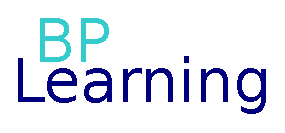
\includegraphics[width=1.5in]{BPLearning.eps}


\vspace*{\fill}

\clearpage %%%%%% PAGE OVER

\thispagestyle{empty}
\vspace*{\fill}
\begin{center}
\hrule
{\LARGE \textsc{\textbf{Electronics for Everyone}}}
\vskip 1\baselineskip
\hrule
\vskip 1\baselineskip
{\Large \textsc{\\ Everything You Need to Get Started with Circuits
}}

\vskip 6\baselineskip

{\LARGE 
	{\textsc{ 
		\hfill by \hspace*{1in} \\ 
		\hfill Jonathan \hspace*{1in} \\ 
		\hfill Bartlett \hspace*{1in} \\
	} }
}

\end{center}

\vspace*{\fill}

\cleardoublepage %%%%% PAGE OVER

\thispagestyle{empty}
\begin{center}

\fbox{
\begin{minipage}{5in}
\begin{center}
\vspace*{0.5in}
\textit{The trick to having good ideas is not to sit around in glorious isolation and try to think big thoughts.  The trick is to get more parts on the table.}
\newline
\newline
---Steven Johnson
\vspace*{0.5in}
\end{center}
\end{minipage}
}

\fbox{
\begin{minipage}{5in}
\begin{center}
\vspace*{0.5in}
\textit{Engineering stimulates the mind.  Kids get bored easily.  They have got to get out and get their hands dirty: make things, dismantle things, fix things.  When the schools can offer that, you'll have an engineer for life.}
\newline
\newline
---Bruce Dickinson
\vspace*{0.5in}
\end{center}
\end{minipage}
}



\end{center}
\vspace*{\fill}

\clearpage

\vspace*{7em}
\begin{minipage}{4in}
\begin{center}
\end{center}
\end{minipage}

\clearpage

\end{titlepage}


\tableofcontents

\mainmatter

\chapter{Introduction}
\label{chapIntro}

Welcome to the world of electronics!  
In the modern world, electronic devices are everywhere, but fewer and fewer people seem to understand how they work or how to put them together.
At the same time, it has never been easier to do so as an individual.
The availability of training tools, parts, instructions, videos, and tutorials available for the home experimenter has grown enormously, and the costs for equipment has dropped to almost nothing.

However, what has been lacking is a good guide to bring students from \emph{wanting} to know how electronic circuits work to actually understanding them and being able to develop their own.
For the hobbyist, there are many guides that show you how to do individual projects, but they often fail to provide enough information for their readers to be able to build projects of their own.
There is plenty of information on the physics of electricity in physics books, but they fail to make the information practical.
There are also books like \booktitle{The Art of Electronics} which are great describing how to put together circuits---but only if you are studying to be an electrical engineer, and also only if you can shell out large amounts of cash.

What has been needed for a long time is a book that takes you from knowing nothing about electronics to being able to build real circuits that you design yourself.
This book combines theory, practice, projects, and design patterns in order to enable you to build your own circuits from scratch.
Additionally, this book is designed entirely around safe, low-current DC power.
We stay far away from the wall outlet in this book to be sure that you have a safe and fun experience with electronics.

Note that this book is primarily written as a textbook for electronics classes for high-school and college students.  
It has problems to be worked, activities to do, and reviews at the end of each chapter.
However, it can also be used as a guide for hobbyists (or wannabe hobbyists) to learn on their own.
If you plan on using this book to learn on your own, we suggest that not only do you read the main parts of the chapter, but that you also do the activities and homework as well.  
The goal of the homework is to train your mind to think like a circuit designer.
If you work through the example problems, it will make analyzing and designing circuits simply a matter of habit.

\section{Working the Examples}

In this book, all examples should be worked out using decimals, not fractions.
This is an engineering course, not a math course, so feel free to use a calculator.
However, you will often wind up with very long strings of decimals on some of the answers.
Feel free to round your answers to a single decimal point.
So, for instance, if I divide 5 by 3 on my calculator, it tells me $1.66666667$.
However, I can just give the final answer as $1.7$.
This only applies to the final answer.  
You need to maintain your decimals while you do your computations.

Also, if your answer is a decimal number that \emph{begins} with zeroes, then you should round your answer to include the first 2--3 nonzero digits.
So, if I have an answer of $0.0000033333333$, I can round that to $0.0000033$.

If you have taken physics or chemistry, and you are familiar with significant digits, you can just round your answers to 3--4 significant digits.

\section{Tools You Will Need}

\fixme{Need to write this - breadboard, jumper wire, resistor, etc.}
\fixme{Need an ``anatomy of a component'' showing a resistor and the leads, as well as an LED and the positive and negative}
\fixme{Need definitions of anode and cathode}
\fixme{Need a forum URL for people with issues}

\chapter{Before We Begin}

I put this chapter at the beginning because it is important and I wanted it easy to find, but you may not know enough to understand all of it.
You can skip over this section and come back to it when you start to do projects in chapter~FIXME.

\section{General Safety Note}
This book deals almost entirely with DC current from small battery sources.  
This current is inherently fairly safe, as small batteries are not capable of delivering the amount of current needed to injure or harm.  
For these projects, you can freely touch wires and work with active circuits without any protection, because the current is incapable of harming you.  

However, please note that if you ever deal with AC current or large batteries (such as a car battery), you must exercise many more precautions than described in this book, because those devices can and will harm or kill you if mishandled.

\section{Safety Guidelines}

Using small-battery DC current is very safe.  Nonetheless, you should employ these safety guidelines, both for your safety and for the safety of your circuit.  The biggest potential problem is with the battery itself, not the electricity.  Batteries are made from potentially toxic chemicals.

Please follow these guidelines, as they will both keep you safe as well as help prevent you from accidentally damaging your own equipment.

\begin{enumerate}
\item If you have any cuts or other open areas on your skin, please cover them. Your skin is where most of your electric protection exists in your body.
\item Before applying power to your circuit, check to be sure you have not accidentally wired in a short circuit between your positive and negative poles of your battery.
\item If your circuit does not behave like you expect it to when you plug in the battery, unplug it immediately and check for problems.
\item If your battery or any component becomes warm, disconnect power immediately.
\item If you smell any burning or smoky smells, disconnect power immediately.
\item Dispose of all batteries in accordance with local regulations.
\item For rechargeable batteries, follow the instructions on the battery for proper charging procedures.
\end{enumerate}

If you follow these common sense rules you should have a fun and safe experience!

\section{Electrostatic Discharge}

If you have ever touched a doorknob and received a small shock, you have experienced electrostatic discharge (ESD).  
ESD is not dangerous to you, but it can be dangerous to your equipment.  
Even shocks that you can't feel may damage your equipment.  
With modern components, ESD is rarely a problem, but nonetheless it is important to know how to avoid it.  
You can skip these precautions if you wish, just know that occasionally you might wind up shorting out a chip or transistor because you weren't careful.  
ESD is also more problematic if you have carpet floors, as those tend to build up static electricity.

Here are some simple rules you can follow to prevent ESD problems:

\begin{enumerate}
\item When storing IC components, store them with the leads enmeshed in conductive foam.  This will prevent any voltage differentials from building up in storage.
\item Wear natural 100\% cotton fabrics.
\item Use a specialized ESD floor mat and/or wrist strap to keep you and your workspace at ground potential.
\item If you don't use an ESD strap or mat, touch a large metal object before starting work.  Do so again any time after moving around.
\end{enumerate}

\section{Using Your Multimeter Correctly}
In order to keep your multimeter functioning, it is important to take some basic precautions.  Multimeters, especially cheap ones, can be easily broken through mishandling.  Use the following steps to keep you from damaging your multimeter, or damaging your circuit with your multimeter:

\begin{enumerate}
\item Do not try to measure resistance on an active circuit.  Take the resistor all the way out of the circuit before trying to measure it.
\item Choose the appropriate setting on your multimeter before you hook it up.
\item Always err on the side of choosing high values first, especially for current and voltage.  Use the high value settings for current and voltage give your multimeter the maximum protection.  If they are too large, it is easy enough to turn them lower.  If you had it set too low, you may have to buy a new multimeter!
\end{enumerate}

%% FIXME - if I add soldering to the book, I also need soldering safety tips


\part{Basic Concepts}

\chapter{What is Electricity?}
\label{electricitybasics}

The first thing to tackle in the road to understanding electronics is to wrap our minds around what electricity is and how it works.
The way that electricity works is very peculiar and unintuitive.
We are used to dealing with the world in terms of physical objects---desks, chairs, baseballs, etc.
Even if we never took a class in physics, we know the basic properties of such objects from everyday experience.
If I drop a rock on my foot, it will hurt.
If I drop a heavier rock, it will hurt more.
If I remove an important wall from a house, it will fall down.

However, for electricity, the only real experience we have is that we have been told to stay away from it.
Sure, we have experience with computers and phones and all sorts of devices, but they give us the result of processing electricity a million times over.
But how does electricity itself work?

\section{Charge}

To answer this question, we need to answer another question first: what \emph{is} electricity?
Electricity is the flow of \glossterm{charge}.
So what is charge?

Charge is a fundamental quantity in physics---it is not a combination (that we know of) of any other quantity.
A particle can be charged in one of three ways---it can be positively charged (represented by a \icode{+} sign), negatively charged (represented by a \icode{-} sign), or be neutrally charged (i.e., have no charge).
Figure~\ref{figChargedParticles} shows what an atom looks like.  
In the center of the atom are larger, heavier particles called \glossterm{protons} and \glossterm{neutrons}.
Protons are positively charged particles, and neutrons are neutrally charged particles.
Together these form the \glossterm{nucleus} of the atom, and determine \emph{which} atom we are talking about.
If you look on a periodic table, the big number of the element refers to how many protons it has in its nucleus, and the smaller number is usually the total number of protons and neutrons (this smaller number is sometimes a decimal because the number of neutrons can change, so it is an average).

\begin{figure}
\caption{Charged Particles in an Atom}
\label{figChargedParticles}
FIXME - need drawing
\end{figure}

Circling around the nucleus are \glossterm{electrons}.
Electrons are negatively charged particles. 
Even though electrons are much smaller and lighter than protons, the amount of negative charge of one electron is equal to the amount of positive charge of one proton.
Positive and negative charges attract each other, which is what keeps electrons contained within the atom.
Electrons are arranged in shells surrounding the nucleus.
The outermost shell, however, is the most important one when thinking about how atoms work.

When we think about individual atoms, we think about them when they are isolated and alone.
In these situations, the number of electrons and protons are equal, making the atom as a whole electrically neutral.
However, especially when atoms interact with other atoms, the configuration of their electrons can change.
If the atoms gain electrons, then they are negatively charged.
If the atoms lose electrons, then they are positively charged.
Free electrons are all negatively charged.

If there are both positively and negatively charged particles moving around, their opposite charges attract one another.
If there is a great imbalance of positive and negative charges, usually you will have a \emph{movement} of some of the charged particles towards the particles of the opposite charge.
This is a \emph{flow} of charge, and is what is referred to when we speak of electricity.

The movement of charge can be either positively-charged particles moving towards negatively-charged ones, or the reverse.
Usually, in electronics, it is the electrons which are moving through a wire, but this is not the only way which charge can move.

Electricity can be generated by a variety of means.
The way that electricity is generated in a battery is that a chemical reaction takes place, but the reactants (the substances that react together) are separated from each other by some sort of medium.  
The positive charges for the reaction move easiest through the medium, but the negative charges for the reaction move easiest through the wire.
Therefore, when the wire is connected, electricity moves through the wire to help the chemical reaction complete on the other side of the battery.

This flow of electric charge through the wire is what we normally think of as electricity.

\begin{sidebar}[Making Your Own Battery]
You can make a simple battery of your own out of three materials: thick copper wire or tubing, a galvanized nail (it \emph{must} be galvanized), and a potato or a lemon.
This battery operates from a reaction between the copper on the wire and the zinc on the outside of the galvanized nail.
The electrons will flow from the zinc to the copper through the wire, while the positive charge will flow within the potato.

To build the battery, you must insert the thick copper and the nail into the potato.  
They should be near each other, but \emph{not touching}.
This is a battery that will produce about 1.2 volts of electricity.
This is not quite enough to light up an LED, but it should register on a multimeter.  
See chapter~FIXME for how to measure voltage with a multimeter.

Different plants will yield different voltages.
You might experiment on this with lemons, strawberries, and other produce items to see what voltages each one produces.

Remember, however, that the potato is not actually supplying the current.
What the potato is doing is creating a barrier so that only the positive charges can flow freely in the potato, and the negative charges have to use the wire.
Note that this can be made even more efficient by boiling the potato first.
\end{sidebar}

\section{Measuring Charge and Current}

Atoms are very, very tiny.
Only in the last few years have scientists even developed microscopes that can see atoms directly.
Electrons are even tinier.
Additionally, it takes a \emph{lot} of electrons moving to have a worthwhile flow of charge.
Individual electrons do not do much on their own---it is only when there are a very large number of them moving that they can power our electronics projects.

Therefore, scientists and engineers usually measure charge on a much larger scale.
The \glossterm{coulomb} is the standard measure of electric charge.
One coulomb is equivalent to the electric charge of about $6,242,000,000,000,000,000$ protons.
If you have that many electrons, you would have $-1$ coulomb.
That's a lot of electrons and protons, and it takes that many to do very much electrical work.
Thankfully, protons and electrons are very, very small.
A typical 9-volt battery can provide about $2,000$ coulombs of charge, which is over $10,000,000,000,000,000,000,000$ electrons (ten thousand billion billion electrons).

However, electricity and electronics are not about electric charge sitting around doing nothing.
Electricity deals with the \emph{flow} of charge.
Therefore, when dealing with electricity, we rarely deal with coulombs.
Instead, we talk about how fast the electrical charge is flowing.
For that, we use \glossterm{amperes}, often called amps, and abbreviated as A.
1 ampere is equal to the movement of 1 coulomb of charge out of the battery each second.

For the type of electronics we will be doing, an ampere is actually a lot of current.
In fact, a full ampere of current can do a lot of physical harm to you, but we don't usually deal with full amperes when creating electronic devices.
Power-hungry devices like lamps, washers, dryers, printers, stereos, and battery-chargers need a lot of current---that's why we plug them into the wall.
Small electronic devices don't usually need so much current.
Therefore, for electronic devices, we usually measure current in \glossterm{milliamperes}, usually called just milliamps, and abbreviated as mA.
The prefix \emph{milli-} means one thousandth of (i.e., $\frac{1}{1000}$ or $0.001$).
Therefore, a milliamp is one thousandth of an amp.
If someone says that there is 20 milliamps of current, that means that there is 0.020 amps of current.
This is important, because the equations that we use for electricity are based on amps, but we are going to be mainly concerned with milliamps.

So, to go from amps to milliamps, multiply the value by $1,000$.
To go from milliamps to amps, divide the value by $1,000$ (or multiply by $0.001$) and give the answer in decimal (electronics always uses decimals instead of fractions).

\begin{exampleprob}
If I were to have $2.3$ amps of electricity, how many milliamps is that?
To go from amps to milliamps, we multiply by $1,000$.  
$2.3 * 1,000 = 2,300$.  
Therefore, $2.3$ amps is the same as $2,300$ milliamps.
\end{exampleprob}

\begin{exampleprob}
If I were to have $5.7$ milliamps of electricity, how many amps is that?
To go from milliamps to amps, we divide by $1,000$.
$5.7 / 1,000 = 0.0057$
Therefore, $5.7$ milliamps is the same as $0.0057$ amps.
\end{exampleprob}

\begin{exampleprob}
Now, let's try something harder---if I say that I am using 37 milliamps of current, how many coulombs of charge has moved after 1 minute?
Well, first, let's convert from milliamps to amps.  
To convert from milliamps to amps, we divide by $1,000$.
$37 / 1000 = 0.037$
Therefore, we have $0.037$ amps.
What is an amp?
An amp is 1 coulomb of charge moving per second.
Therefore, we can restate our answer as being $0.037$ coulombs of charge moving each second.

However, our question asked about how much has moved after 1 \emph{minute}.
Since there are $60$ seconds in each minute, we can multiply $0.037$ by $60$ for our answer.
$0.037 * 60 = 2.22$
So, after 1 minute, 37 milliamps of current moves $2.22$ coulombs of charge.
\end{exampleprob}

\section{AC vs. DC Current}

You may have heard the terms AC or DC when people talk about electricity.
What do those terms mean?
In short, DC stands for \glossterm{direct current} and AC stands for \glossterm{alternating current}.
So far, our descriptions of electricity have dealt mostly with DC current.
With DC current, electricity makes a route from the positive terminal to the negative.
It is the way most people envision electricity.
It is ``direct.''

However, DC current, while great for electronics projects, very quickly loses power over long distances.
If we were to transmit current that simple flows from the positive to the negative throughout the city, we would have to have power stations every mile or so.

So, instead of sending current in through one terminal and other through another, with alternating current, the positive and negative sides make a complete switch (both back and forth) 50--60 times per second.
So, the electrons switch back and forth, over and over again, which direction they are moving.
It is like someone is pushing and pulling current back-and-forth.
In fact, at the generator station, that is exactly what is going on!
This may seem strange, but this push and pull action allows much easier power generation and allows much more power to be delivered over much longer distances.

AC current such as the current that comes out of a wall socket is much more powerful than we require for our projects here.
In fact, converting high-power AC current to low-power DC voltage used in electronic devices is an art in itself.
This is why companies charge so much money for battery chargers---it takes a lot of work to get one right!

Now, not all AC current is like this.  
We call this current AC ``mains'' current, because it comes from the power mains from the power stations.
It is supposed to operate at about 120 volts and the circuits are usually rated for about 15--30 amps (that's 15,000--30,000 milliamps).
That's a lot of electricity!

In addition to AC mains current, there are also AC currents which we will call AC ``signal'' current.
These currents come from devices like microphones.
They are AC because they do alternate.
When you speak, your voice vibrates the air back-and-forth.
A microphone converts these air vibrations into small vibrations of electricity---pushing and pulling a small electric current back and forth.
However, these AC currents are so low-powered as to be almost undetectable.
They are so small, we have to actually amplify these currents just to work with them using our DC power!

So, in short, while we will do some work with AC voltages later in the book, all of our projects will be safe, low-power projects.
We will often touch wires with our projects active, or use multimeters to measure currents and voltages in active circuits.
This is perfectly safe for battery-operated projects.
But \emph{do not} attempt these same maneuvers for anything connected to your wall outlet unless you are properly trained.

\section{Which Way Does Current Flow?}

One issue that really bungles people up when they start working with electronics is figuring out which way that electrical current flows.
You hear first that electrical current is the movement of electrons, and then you hear that electrons move from negative to positive.
So, one would naturally assume that current flows from negative to positive, right?

Good guess, but no.
Current is not the flow of physical stuff like electrons, but the flow of \emph{charge}.
So, when the chemical reaction happens in the battery, the positive side gets positively charged.
The electrons are a negative charge that moves toward the positive charge.
The positive charge is just as real as the electron charge, even though physical stuff isn't moving.

Think about it this way.
Have you ever used a vacuum cleaner?
Let's say we are building a vacuum cleaner.
Where do you start?
Usually, you start at the inside where the suction happens and then trace the flow of suction through the tubes.
Then, at the end of the tube, the dust comes into tube.

Engineers don't trace their systems from the dust to the inside, they trace their systems from the suction on the inside out to the dust particles on the outside.
Even though it is the dust that moves, it is the suction that is interesting.

Likewise, for electricity, we usually trace current from positive to negative even though the electrons are moving the other way.
The positive charge is like the suction of a vacuum, pulling the electrons in.
Therefore, we want to trace the flow of the vacuum from positive to negative, even though the dust is moving the other way.

The idea that we trace current from positive to negative is often called \glossterm{conventional current flow}.
It is called that way because we conventionally think about circuits as going from the positive to the negative.
If you are tracing it the other way, that is called \glossterm{electron current flow}, but it is rarely used.

\reviewsection

In this chapter, we learned:

\begin{enumerate}
\item Electric current is the flow of charge.
\item Charge is measured in coulombs.
\item Electric current flow is measured in coulombs per second, called amperes or amps.
\item A milliampere is one thousandth of an ampere.
\item In an atom, protons are positively charged, electrons are negatively charged, and neutrons are neutrally charged.
\item Batteries work by having a chemical reaction which causes electricity to flow through wires.
\item In DC current, electricity flows continuously from positive to negative.
\item In AC current, electricity flows back and forth, changing flow direction  many times every second.
\item Even though electrons flow from negative to positive, in electronics we usually think about circuits and draw circuit charges as flowing from positive to negative.
\item AC mains current (the kind in your wall outlet) is dangerous, but battery current is relatively safe.
\item Small signal AC current (like that generated by a microphone) is not dangerous, either.
\end{enumerate}

\applysection


\begin{enumerate}
\item If I have 56 milliamps of current flowing, how many amps of current do I have flowing?
\item If I have 1,450 milliamps of current flowing, how many amps of current do I have flowing?
\item If I have 12 amps of current flowing, how many milliamps of current do I have flowing?
\item If I have 0.013 amps of current flowing, how many milliamps of current do I have flowing?
\item If I have 125 milliamps of current flowing for one hour, how many coulombs of charge have I used up?
\item What is the difference between AC and DC current?
\item In AC mains current, how often does the direction of current go back and forth?
\item Why is AC used instead of DC to deliver electricity within a city?
\item In working with electronic devices, do we normally work in amps or milliamps?
\end{enumerate}


\chapter{Voltage and Resistance}

In the previous chapter we learned about current, which is the rate of flow of charge.
In this chapter we are going to learn about two other fundamental electrical quantities---\glossterm{voltage} and \glossterm{resistance}.
These two quantities are the ones that are usually the most critical to building effective circuits.

Current is important because limiting current allows us to preserve battery life and protect precision components.
Voltage, however, is usually the quantity that has to be present to do any work within a circuit.

\section{Picturing Voltage}

What is voltage?
Voltage is the amount of power each coulomb of electricity can deliver.
If you have a one coulomb of electricity at 5 volts and I have one coulomb of electricity at 10 volts, that means that my coulomb can deliver twice as much power as yours.

A good analogy to electronics is the flow of water.
When comparing water to electricity, \emph{coulombs} are a similar unit to \emph{liters}---coulombs measure the amount of electrical charge present just like a liter is the amount of water stuff present.
Both charge and water both flow.
In water, we can measure the flow of a current of a stream in liters-per-second.
Likewise, in electronics, we measure the flow of charge through a wire in coulombs-per-second, called amperes.

Now, I want you to image the end of a hose containing water.
Normally, the water just falls out of the hose, especially if the hose is just sitting on the ground.
That hose just sitting on the ground is like a current with zero volts---each unit of water or charge is just not doing that much.

Let's pretend we added a spray nozzle to the hose.
What happens now?
Water shoots out of the nozzle.
We haven't added any more water---it is actually the same amount of current flowing.
Instead, we increased the pressure on the water, which is just like increasing the voltage on an electric charge.
By increasing the pressure, we changed the amount of work that each liter of water is available to perform.
Likewise, when we increase voltage, we change the amount of work that each coulomb of electricity can do.

One way we might measure the pressure of water coming out of a hose is to measure how far up it can shoot out of the hose.
By doubling the pressure of the water, we can double how far out of the hose it can shoot.
Similarly, with voltages, large enough voltages can actually jump air gaps across circuits.
However, to do this, it takes a lot of voltage---about 30,000 volts per inch of gap.
If you have been shocked by static electricity, though, this is what is happening!
The power of the charge was extreme (thousands of volts), but the amount of charge in those shocks are so small that it doesn't harm you (about 0.00000001 coulombs).

\section{Volts are Relative}

While charge and current are fairly concrete ideas, voltage is a much more relative idea.
You can actually never measure voltage absolutely.
All voltage measurements are actually relative to other voltages.
That is, I can't actually say that my electric charge has exactly 1, 2, 3, or whatever volts.
Instead, what I have to do is say that one charge is however many volts more or less than another charge.
So, let's take a 9-volt battery.
What that means is not that the battery is 9 volts in any absolute sense, but rather that there is a 9-volt \emph{difference} between the charge at the positive terminal and the charge at the negative terminal.
That is, the pressure with which charge is trying to move from the positive terminal to the negative terminal is 9 volts.

\section{Relative Voltages and Ground Potential}

When we get to actually measuring voltages on a circuit, we will only be measuring voltage \emph{differences} on the circuit.
So, I can't just put a probe on one place on the circuit, I have to put my probe on two different places on the circuit and measure the voltage difference (also called the \glossterm{voltage drop}) between those two points.

However, to simplify calculations and discussions, we usually choose some point on the circuit to represent ``zero volts.''
This gives us a way to standardize voltage measurements on a circuit, since they are all given relative to the same point.
In theory this could be any point on the circuit, but, usually, we choose the negative terminal on the battery to represent zero volts.

This ``zero point'' goes by several names, the most popular of which is \glossterm{ground} (often abbreviated as \glossterm{GND}).
It is called the ground because, historically, the physical ground has often been used as a reference voltage for circuits.
Using the physical ground as the zero point allows you to also compare voltages between circuits with different power supplies.
However, in our circuits, when we refer to the ground, we are referring to the negative terminal on the battery, which we are designating as zero volts.
If we designate any other part of the circuit as a ground, we will let you know.  % FIXME - need to pull or clarify this depending on what is in the final version of the book

Another, lesser-used term for this designated zero volt reference is the \glossterm{common} point.
Many multimeters label one of their electrodes as \glossterm{COM}, for the common electrode.
When analyzing a circuit's voltage, this electrode would be connected to whatever your zero-volt point is.

This ``ground'' analogy also makes sense with our water hose analogy.
Remember that a voltage is the potential for a charge to do work.
What happens to water after it lands on the ground?
By the time the water from my hose lands on the ground, it has lost all its energy.
It is just sitting there.
Sure, it may seep or flow around a bit, but nothing of consequence.
All of its ability to do work---to move quickly or to knock something over---has been drained.
It is just on the ground.
Likewise, when our electric charge is all puttered out, we say that it has reached ``ground potential.''

So, even though we could designate any point as being zero, we usually designate the negative terminal of the battery as the zero point, indicating that by the time electricity reaches that point, it has used up all of its potential energy---it now has zero volts.

\section{Voltage and Resistance}



\chapter{Your First Circuit}
\label{chapFirstCircuit}

In the last two chapters we have learned about the fundamental units of electricity---charge, current, voltage, and resistance.
In this chapter, we are going to put this information to use in a real circuit.

\section{Circuit Requirements}

For a circuit to function properly, you usually need several things:

\begin{enumerate}
\item A source (usually providing a constant voltage) which provides electricity for your circuit
\item A network of wires and components that ultimately lead from your voltage source to ground (which is usually the negative terminal on the battery)
\item Some amount of resistance in your circuit
\end{enumerate}

We need the source because, without a source, we don't have any power to move electricity around!
If we have a circuit, but no source, it will just sit there.
In our circuits, batteries will usually provide the power we need.

We need the wires because, unless we provide a \emph{complete pathway} from a higher voltage to a lower voltage, the electricity won't move.  
If we want electricity to move, we have to make a pathway from a higher voltage to a lower voltage.
Without this pathway, we have what is known as an \glossterm{open circuit}.
No electricity flows in an open circuit.

However, in addition to the wires, we must also have resistance.
Without resistance, the current would be too high.
It would be so high that it would immediately drain your battery, and likely destroy all of your components that you have connected.
You can actually see this using Ohm's law.
If we have a 10-volt source with no resistance, the current is given by the equation $I = V / R = 10 / 0$.
Dividing by zero gives you, essentially, infinite current.
Now, wires and batteries themselves have some resistance, so the current wouldn't be infinite, but it would be very, very large and would quickly drain your battery and destroy any sensitive components you had connected.
Therefore, every pathway from the positive side of the battery to the negative \emph{must} have some amount of resistance.
When a pathway from positive to negative occurs without resistance, this is known as a \glossterm{short circuit}.

In other words, to accomplish real tasks with electricity, we must control its flow.  
If it doesn't flow (as in an open circuit), it can't do anything.
If it flows without resistance (as in a short circuit), it does damage rather than work.
Therefore, the goal of electronics is to provide a controlled route so that the power of electricity does the things we want it to do on its way from positive to negative.

\section{Basic Components}

The first circuits that we will build will only use three basic types of components:
\begin{itemize}
\item Batteries (9-volt)
\item Resistors
\item LEDs
\end{itemize}

As we have discussed before, batteries provide a constant amount of voltage between the positive and negative terminals.
A 9-volt battery, therefore, will always have a 9-volt difference between the positive and negative terminals.

A resistor is a device that, as its name implies, adds resistance to a circuit.
Resistors have colors that indicate how much resistance they add to the circuit.
You don't need to know the color codes yet, but if you are curious you can see the resistor datasheet in Appendix~\ref{appSimplifiedDatasheets}.
So, if we want to add 100\si{\ohm} to our circuit, we just find a resistor with a value of 100\si{\ohm}.
Resistors are not the only devices that add resistance to a circuit, but they are usually what are used when you want to add a fixed amount of resistance.
Resistors have two sides, but they both function identically---there is no backwards or forwards for a resistor.  
You can put them in your circuit either way and they will function just fine.

Of the components in this section, the LED is probably the strangest.
LED stands for light-emitting diode.
A diode is a component that only allows current to flow in one direction.
It blocks the flow of electricity in the other direction.
However, more importantly, LEDs emit light when current passes through them.
However, LEDs do not resist current, so they must be used with a resistor to limit the amount of current flowing through them (most of them will break at 20--30 milliamps).
Also, since LEDs only allow current to flow one way, they have to be wired in the right direction.
The legs of an LED are different lengths.
The longer leg of the LED should be on the more positive side of the circuit.

Most of your components (especially your resistors) come with very long legs.
You can feel free to bend or cut these legs however you please to better fit in your circuit.
However, on LEDs (and any other component where leg length matters), be sure to keep the longer legs longer so you don't get confused about which leg is the positive leg.

\section{Creating Your First Circuit}

Now we will put together a simple first circuit.
What you will need is:
\begin{itemize}
\item 1 9-volt battery
\item 1 red LED (other colors will work, too)
\item 1 500\si{\ohm} resistor (anything from 400 ohms to 1,000 ohms should work)
\end{itemize}

Even if you can't read the color codes on the resistor, you should be able to buy them with the value you want.
To make this circuit, take one leg of the resistor and twist it together with the \emph{short} leg of the LED.
It should look like Figure~\ref{figLEDWrapped}.

\begin{figure}
\caption{Wrapping the Resistor around the LED's Short Leg}
\label{figLEDWrapped}
\fixme{Need picture here}
\end{figure}

Now, take the long leg of the LED and touch it to the positive terminal of the battery.
Nothing happens---why not?
Nothing happens because even though we have connected the wires to the positive side of the battery, the electricity has nowhere to go to.
We have an open circuit because there is not a complete path from positive to negative.

Now, touch the long leg of the LED to the battery and, at the same time, touch the unattached end of the resistor to the battery.
The LED should give a nice glow of its color.
Congratulations---you have built your first circuit!

Even though we can't see the electricity moving, I hope you can see how it will flow through the circuit.
We can trace the current flow from the positive terminal of the battery through the LED.
The resistor limits the amount of current flowing through the circuit, and therefore through our LED (the resistor can actually go on either side of the LED, it will limit the flow no matter which side it is on).
Without the resistor, the battery would easily go over the 30 milliamp rating of our LED and it would no longer work.  
If you connected it without a resistor, you might see it turn on for a moment and then very quickly turn off, and then it would never work again.
If you have an extra LED you can try this out if you want.
It is not dangerous it will just cost you the price of an LED.

If your LED is backwards, no current will flow at all. 
It won't hurt the LED, but it won't turn on unless it is oriented in the right direction.

\section{Adding Wires}
\label{secWireRule}

We are not going to physically add wires to our circuit at this time, but I did want to make a note on wires.
Changing the lengths of wires will not affect our circuits in any way.
For some high-precision circuits, or some very long wires, the length of a wire will have some effect on these circuits.
We are not doing any high-precision circuits, and our wire lengths are all less than a meter.
Therefore, for the electronics we are doing, we can totally ignore wire length.

Therefore, if we connected our components using wires rather than directly wrapping their legs around each other directly, it would have no effect on the circuit at all.
What is important is not the wires but the connections---what components are connected together and how are they connected.
The length of wire used to connect them is not important.

\section{Drawing Circuits}

So far, we have only described circuits in words or by showing you pictures.
This, however, is a lousy way of describing circuits.
In complicated circuits, trying to trace the wires in a photograph is difficult.
If you wanted to draw a circuit that you wanted built, you would have to be an artist to render it correctly.
Likewise, reading through text describing a circuit takes a long time and is easy to get lost for large circuits.

Therefore, in order to communicate information about how a circuit is put together in a way that is easy to read and write, engineers have developed a way of drawing circuits called \glossterm{circuit diagrams} or \glossterm{electronic schematics} (often shortened to just \emph{diagram} or \emph{schematic}).
In a circuit diagram, each component is represented by an easy-to-draw symbol that helps you remember what the component does.
Figure~\ref{figBasicDiagramSymbols} shows the symbols for the components we have used so far.
Note that everybody draws the symbols slightly differently, and some components have more than one symbol.
However, these are the symbols we will use in this book.
For more symbols, see Appendix~\ref{appendixSymbols}.

\begin{figure}
\caption{Basic Component Diagram Symbols}
\label{figBasicDiagramSymbols}
\begin{center}
\begin{tabular}{M{0.1\linewidth} | M{0.12\linewidth} | m{0.6\linewidth}}
\textbf{Symbol} & \textbf{Component} & \textbf{Description} \\
\includegraphics[scale=0.125]{BatterySymbol.png} & Battery & A battery is represented by a long line and a short line stacked on top of each other.  Sometimes, there are two sets of long and short lines.  The long line is the positive terminal and the short line is the negative terminal (which is usually used as the ground). \\ \hline
\includegraphics[scale=0.25]{ResistorSymbol.pdf} & Resistor & A resistor is represented by a sharp, wavy line with wires coming out of each side. \\ \hline
\includegraphics[scale=0.125]{LEDSymbol.png} & LED & An LED is represented by an arrow with a line across it, indicating that current can flow from positive to negative in the direction of the arrow, but it is blocked going the other way.  The LED symbol also has two short lines coming out of it, representing the fact that it emits light. \\
\end{tabular}
\end{center}
\end{figure}

Then, the components are connected together using lines to represent the wires and connections between the components.

Therefore, we can redraw our original circuit using these symbols like you see in Figure~\ref{figCircuitBasicLED}.

\begin{figure}
\caption{Basic LED Circuit Drawn as a Diagram}
\label{figCircuitBasicLED}
\centering
\includegraphics[scale=0.125]{CircuitBasicLED.png}
\end{figure}

Notice that each of our components are laid out on the diagram with wires connecting them.
Remember that it doesn't matter if we have very long wires, very short wires, or if the components are directly placed end-to-end---the resulting circuits will operate identically.
Also notice that each component is labeled (R1 and D1) because, as we make more complicated circuits, it is important to be able to refer back to them.

It does not matter in a diagram which way you have your components turned, how long or short your wires are, or what the general spacing looks like.
When you actually wire it, all of those things will change.
The important part of a circuit diagram is to convey to the reader what the parts are, how they are connected, and what the circuit does in the way that is easiest to read.

For instance, all of the circuits in Figure~\ref{figCircuitLEDAlt} are equivalent to the circuit in Figure~\ref{figCircuitBasicLED}, they are just drawn differently.

\begin{figure}
\caption{Alternative Ways of Drawing the Basic LED Circuit}
\centering
\label{figCircuitLEDAlt}
\includegraphics[scale=0.08]{CircuitLEDAlt}
\end{figure}

For consistency, I like to draw all of my batteries to the left of the drawing with the positive side on top.
By keeping the battery positive-side-up, components with higher voltage are usually closer to the top, and components with lower voltages are usually closer to the bottom, with the ground (i.e., zero volts) coming back into the negative terminal.
I also try to make my wire lines as simple as possible in order to make following them easier.

By keeping some amount of consistency, it is easier to look at a drawing and see what it happening.

\section{Drawing the Ground}

Remember that for electricity to move, every circuit must be fully connected from the positive side to the negative side.
That means that in larger circuits there are numerous connections that come from the positive or go back to the ground/negative.
Because of this, a special symbol has been adopted to refer to the ground point in a circuit.
This symbol, the ground symbol, has three lines, each shorter than the next.
Every point on a circuit that has this symbol connected to it is connected to each other (usually they are all connected to the negative side of the battery).

Therefore, the circuit in Figure~\ref{figCircuitBasicLEDGround} is the same circuit as before, just drawn using the ground symbol.
Since every point with the ground symbol are all connected together, using this symbol on both the negative terminal and the negative side of the LED means that they are wired together.

This doesn't help us a lot for this circuit (and, in fact, it makes it a little less easy to read).  
However, in complex circuits, it is much easier to write the ground symbol than trying to have twenty lines drawn back to the negative terminal.

\simplegraphicsfigure{Basic LED Circuit Drawing Using the Ground Symbol}{CircuitBasicLEDGround}{0.08}

Additionally, the same is true with the positive side of the battery.
Many components require a direct connection to a specific voltage to work correctly.
These are usually marked with just a disconnected wire with the end of the wire marking what voltage it requires.
We make less use of that symbol in this book than the ground symbol, but it does come in handy sometimes.

So, using both the voltage source and the ground symbols, we could rewrite the same circuit again in the manner shown in Figure~\ref{figCircuitBasicLEDPosGround}.
This circuit, again, is not \emph{wired} any differently than before.
We are just \emph{drawing} it differently.
For this circuit, it doesn't matter, but in more complex circuits, if we need a specific voltage at a specific location, this symbol tells us to put it there.

\simplegraphicsfigure{Simple LED Circuit Using Positive and Ground Symbols}{CircuitBasicLEDPosGround}{0.08}

\reviewsection

In this chapter, we learned:

\begin{enumerate}
\item Every circuit requires a source of power (usually a battery), wires and components, some amount of resistance, and a complete path back to the negative side of the power source.
\item An open circuit is one that does not connect back to the negative side (and thus does not provide any electricity), and a short circuit is one that connects back to the negative side without any resistance (and thus overwhelms the circuit with current).
\item Batteries supply a fixed voltage between its two terminals.
\item A resistor provides a fixed resistance (measured in ohms) within your circuit.
\item An LED allows current to flow in only one direction, gives off light when current is flowing, but is destroyed when the current goes above 20--30 milliamps.
\item The longer leg of the LED should be on the positive side of the circuit.
\item Wires on a circuit can be almost any length (from zero to a few meters) without changing the functionality of the circuit.
\item A circuit diagram is a way of drawing a circuit so that it is easy to read and understand what the circuit is doing.
\item Each component has its own symbol in a circuit diagram.
\item Every component labeled with the ground symbol is connected together, usually at the negative side of the battery.
\item Voltage sources can be similarly labeled by a wire connected on one side labeled with the voltage that it is supposed to be carrying.
\end{enumerate}

\applysection


\textbf{Special Note} - In the problems below, since we have not yet studied LED operation in-depth, we are ignoring the electrical characteristics of the LED and just focusing on the resistor.  
If you know how to calculate the circuit characteristics using the LED, please ignore it anyway for the purpose of these exercises.

\begin{enumerate}
\item 
\question{Calculate the amount of current running in the circuit you built in this chapter using Ohm's law.  Since Ohm's law gives the results in amps, convert the value to milliamps.}
\solution{$18\mymamp$}
\explanation{We can use Ohm's Law (Equation~\ref{ohmequationi}) to find the current running through this circuit:
\begin{align*}
I &= V / R \\
  &= 9 / 500 \\
  &= 0.018
\end{align*}
Therefore, the circuit produces $0.018\myamp$ of current.  Multiply by $1,000$ to get milliamps and we get $18\mymamp$ of current.
}
\item 
\question{Let's say that the minimum amount of current needed for the LED to be visibly on is 1 milliamp.  What value of resistor would produce this current?}
\solution{$9,000\myohm$}
\explanation{To find this out, we just need to use Ohm's law to find the necessary resistance using Equation~\ref{ohmequationr}.  However, Ohm's law is given in amps, so we need to convert $1\mymamp$ to amps.  $1\mymamp = 0.001\myamp$.  Therefore, we can calculate the resistor value with the following:
\begin{align*}
R &= V / I \\
  &= 9 / 0.001 \\
  &= 9,000
\end{align*}
We would need $9,000\myohm$ of resistance to reduce the current to 1 milliamp.
}
\item 
\question{Let's say that the maximum amount of current the LED can handle is 30 milliamps.  What value of resistor would produce this current?}
\solution{$300\myohm$}
\explanation{To solve this problem we need to use Ohm's law, but first we need to convert milliamps into amps to do this.  $30\mymamp = 0.03\myamp$.  Now we can use Equation~\ref{ohmequationr} to solve:
\begin{align*}
R &= V / I \\
  &= 9 / 0.03 \\
  &= 300
\end{align*}
Therefore, a resistor of $300\myohm$ would produce this current.
}
\item 
\question{Draw a circuit diagram of a short circuit.}
\solution{This is an open-ended question, so a number of results are possible.  For it to be successful, you must be able to trace a path from the positive terminal of the battery to the negative terminal of the battery without going through a resistor.}
\item 
\question{Take the circuit drawing in this chapter, and modify it so that it is an open circuit.}
\solution{This is an open-ended question, so a number of results are possible.  For it to be successful, you must not be able to trace \emph{any} path from the positive terminal of the battery to the negative terminal of the battery.}
\item 
\question{Draw a circuit with just a battery and a resistor.  Make up values for both the battery and the resistor and calculate the amount of current flowing through.}
\solution{This is an open-ended question, but the circuit should be neither a short circuit nor an open circuit.  Equation~\ref{ohmequationi} should be used to calculate the amount of current flowing through the circuit.}
\end{enumerate}


\chapter{Series and Parallel Circuits}

In the Chapter~\ref{chapFirstCircuit} we looked at our very first circuit and how to draw it using a circuit diagram.
In this chapter, we are going to look at different ways components can be hooked together and what they mean for your circuit.

\section{A Series Circuit}

The circuit built in Chapter~\ref{chapFirstCircuit} is considered a \glossterm{series circuit} because all of the components are connected end-to-end, one after another.
In a series circuit, there is only one pathway for the current to flow, making analyzing the circuit fairly simple.

It does not matter how \emph{many} components are connected together---as long as all of the components are connected one after another, the circuit is considered a series circuit.


\appendix

\chapter{Glossary}
\label{chapGlossary}

\begin{description}
\item[AC current] See \emph{alternating current}.
\item[AC mains current] This is the type of current that is supplied to your house by the public utility companies.  This is usually 120 volts AC and cycles back and forth 50--60 times per second.
\item[AC signal current] This is the type of current usually picked up by a microphone or antenna.  It has very low current and usually must be amplified before processing.
\item[alternating current]
\item[amp] A shorthand way of saying ampere.  See \emph{ampere}.
\item[ampere] An ampere is a measurement of the movement of charge.  It is equivalent to one coulomb of charge per second moving past a given point in a circuit.
\item[anode]
\item[cathode]
\item[charge] Charge is a fundamental quantity in physics.  A particle can be positively charged (like a proton), negatively charged (like an electron), or neutrally charged (like a neutron).  Charge is measured in coulombs.
\item[closed circuit] A circuit is closed if there is a complete pathway from the positive to the negative.
\item[conventional current flow]
\item[coulomb] A coulomb is a quantity of electric charge.  One coulomb is roughly equivalent to the charge of $6.242×10^18$ protons.  The same number of electrons produces a charge of $-1$ coulomb.  Coulombs are represented by the symbol C.
\item[DC current] See \emph{direct current}.
\item[direct current]
\item[electron current flow]
\item[electron] A negatively-charged particle that is usually on the outside of an atom.
\item[milliamp] A short way of saying milliampere.  See \emph{milliampere}.
\item[milliampere] One thousandth of an ampere.  See \emph{ampere}.
\item[neutron] An uncharged particle in the nucleus of an atom.
\item[nucleus] The nucleus is the part of the atom where protons and neutrons reside. 
\item[open circuit] An open circuit is a condition where there is no electrical pathway for the current to flow.  See also \emph{closed circuit}, \emph{short circuit}.
\item[parallel circuit] A circuit is a parallel circuit if one or more components are arranged into multiple branches.
\item[proton] A positively-charged particle in the nucleus of an atom.
\item[resistance] Resistance measures how much a component resists the flow of electricity.  Resistance is measured in ohms (\si{\ohm}).
\item[series circuit] A series circuit is a circuit or part of a circuit where all of the components are connected one after another.
\item[short circuit] A short circuit is what happens when the current pathway has no resistance from the positive to the negative.
\end{description}

\chapter{Finding Component Values}

Since electronic components are so small and oddly-shaped, manufacturers have had to come up with some strange systems to let you know what values your components hold.
This appendix will tell you how, in most cases, to tell the values of different components.

\section{Resistors}
\label{appendixResistorValues}

\chapter{Electronics Symbols}
\label{appendixSymbols}

\begin{center}
\begin{tabular}{M{0.1\linewidth} | M{0.12\linewidth} | m{0.6\linewidth}}
\textbf{Symbol} & \textbf{Component} & \textbf{Description} \\
\includegraphics[scale=0.125]{BatterySymbol.png} & Battery & A battery is represented by a long line and a short line stacked on top of each other.  Sometimes, there are two sets of long and short lines.  The long line is the positive terminal and the short line is the negative terminal (which is usually used as the ground). \\ \hline
\includegraphics[scale=0.125]{ResistorSymbol.png} & Resistor & A resistor is represented by a sharp, wavy line with wires coming out of each side. \\ \hline
\includegraphics[scale=0.125]{LEDSymbol.png} & LED & An LED is represented by an arrow with a line across it, indicating that current can flow from positive to negative in the direction of the arrow, but it is blocked going the other way.  The LED symbol also has two short lines coming out of it, representing the fact that it emits light. \\
\end{tabular}
\end{center}



\end{document}

